\chapter{Metodologia badań i projekt rozwiązania}

Rozdział opisuje sposób przejścia od problemu sformułowanego we wstępie do powtarzalnego eksperymentu. Przedstawiono w nim źródło danych, kolejne etapy ich przygotowania, definicję operacyjnej etykiety FTP, warianty cech oraz zasady podziału i oceny modeli.

Opracowane rozwiązanie ma charakter prototypowego systemu analitycznego. Jego zadaniem jest przekształcenie surowych danych telemetrycznych z treningów kolarskich w tabelaryczny zestaw cech, przygotowanie etykiet FTP oraz ocena modeli regresyjnych. System realizuje potok Extract--Transform--Load (ETL), obejmujący pozyskanie danych, ich filtrację, ekstrakcję cech oraz przygotowanie zbioru do eksperymentów uczenia maszynowego.

\section{Architektura potoku przetwarzania}

Przetwarzanie danych zaprojektowano jako sekwencję etapów, z których każdy ma określone wejście i wyjście. Rozdzielenie odpowiedzialności ułatwia kontrolę jakości, ponowne uruchamianie wybranego fragmentu procesu oraz identyfikację miejsca, w którym powstał ewentualny błąd. Ogólny przebieg potoku obejmuje:
\begin{enumerate}
    \item pozyskanie archiwów ZIP zawierających historie treningowe użytkowników;
    \item kontrolowane rozpakowanie kolejnych paczek danych;
    \item identyfikację i odczyt plików \texttt{.csv} opisujących sesje;
    \item przetworzenie szeregów czasowych oraz agregację cech na poziomie aktywności;
    \item utworzenie heurystycznej etykiety \texttt{ftp\_label};
    \item zastosowanie filtra wartości FTP i zapis tabelarycznego datasetu;
    \item przygotowanie wariantów cech A, B i C;
    \item trening modeli oraz ewaluację na osobniczo wydzielonym zbiorze testowym.
\end{enumerate}

Taki układ oddziela etap danych surowych od etapu modelowania. Eksperymenty uczenia maszynowego nie operują bezpośrednio na plikach źródłowych, lecz na przygotowanym datasecie sesji. Dzięki temu porównanie wariantów cech i modeli odbywa się na tej samej podstawie materiałowej, a ponowne uruchomienie eksperymentu nie wymaga każdorazowego przetwarzania wszystkich archiwów.

Całościowy przepływ danych od repozytorium źródłowego do interpretacji wyników przedstawiono na rysunku~\ref{fig:pipeline_architecture}. Diagram porządkuje etapy przygotowania telemetrii, tworzenia wariantów eksperymentalnych, separacji zawodników oraz oceny modeli regresyjnych.

\begin{figure}[htbp]
\centering
\begin{tikzpicture}[
  node distance=0.28cm,
  boxstep/.style={draw, rounded corners, align=center, minimum height=0.72cm, text width=11.7cm, fill=gray!8},
  branch/.style={draw, rounded corners, align=center, minimum height=1.12cm, text width=11.7cm, fill=blue!7},
  arrow/.style={-{Stealth[length=2.4mm]}, thick}
]
\node[boxstep] (source) {\textbf{1. Dane źródłowe:} GoldenCheetah OpenData};
\node[boxstep, below=of source] (raw) {\textbf{2. Przygotowanie danych:} pobranie danych surowych i ekstrakcja aktywności z plików źródłowych};
\node[boxstep, below=of raw] (features) {\textbf{3. Kontrola jakości i inżynieria cech:} czyszczenie danych oraz budowa cech telemetrycznych};
\node[boxstep, below=of features] (label) {\textbf{4. Budowa etykiety:} heurystyczna wartość FTP wyznaczona z maksymalnej średniej mocy 20-minutowej};
\node[branch, below=of label] (variants) {\textbf{5. Warianty eksperymentalne:} A z \texttt{mmp\_20min}; B bez bezpośredniego leakage; C bez cech \texttt{mmp\_*}};
\node[boxstep, below=of variants] (split) {\textbf{6. Podział danych:} \texttt{GroupShuffleSplit} po \texttt{athlete\_id}};
\node[boxstep, below=of split] (models) {\textbf{7. Trenowanie modeli:} Ridge Regression, Random Forest i XGBoost};
\node[boxstep, below=of models] (metrics) {\textbf{8. Ewaluacja i interpretacja:} MAE, RMSE, $R^2$ oraz rekomendacje praktyczne};

\draw[arrow] (source) -- (raw);
\draw[arrow] (raw) -- (features);
\draw[arrow] (features) -- (label);
\draw[arrow] (label) -- (variants);
\draw[arrow] (variants) -- (split);
\draw[arrow] (split) -- (models);
\draw[arrow] (models) -- (metrics);
\end{tikzpicture}
\caption{Schemat architektury potoku analitycznego}
\label{fig:pipeline_architecture}
\figsource{Opracowanie własne.}
\end{figure}

Diagram ten pełni funkcję przewodnika po metodologii pracy: porządkuje kolejne kroki od surowej telemetrii do ewaluacji modeli. Pokazuje, że przygotowanie danych i separacja zawodników stanowią kluczowe etapy przed samym modelowaniem regresyjnym.

\section{Charakterystyka źródeł danych}

Podstawę materiałową badań stanowiły zanonimizowane dane treningowe ze zbioru GoldenCheetah OpenData udostępnionego w ramach projektu Open Science Framework (OSF) \parencite{osf_goldencheetah_opendata}. Zastosowanie otwartego repozytorium pozwoliło objąć analizą zawodników o zróżnicowanym poziomie wytrenowania oraz sesje rejestrowane w warunkach terenowych.

Użytkownicy GoldenCheetah OpenData nie muszą być reprezentatywni dla całej populacji kolarzy: korzystają z określonego oprogramowania, rejestrują aktywności w określony sposób i zdecydowali się udostępnić dane w otwartym repozytorium. Ograniczenie to dotyczy możliwości uogólniania wyników na inne populacje, a nie użyteczności zbioru w ramach przeprowadzonego badania.

Wykorzystany zbiór GoldenCheetah OpenData ma charakter wtórny i obejmuje dane treningowe udostępnione w postaci zanonimizowanych archiwów aktywności. Analiza nie obejmowała danych osobowych zawodników ani prób ich identyfikacji, a identyfikatory sportowców traktowano wyłącznie jako techniczne grupy potrzebne do kontroli podziału danych i ograniczenia ryzyka przecieku informacji osobniczej.

Po kontrolowanym przetwarzaniu wykorzystano 781 archiwów ZIP zawierających dane użytkowników oprogramowania GoldenCheetah. Surowe dane wejściowe miały postać szeregów czasowych opisujących między innymi moc, tętno oraz kadencję. Skrypt ekstrakcji przekształcał pliki \texttt{.csv} zagnieżdżone w archiwach ZIP w tabelę, w której pojedynczy rekord odpowiada jednej sesji treningowej.

Pojedyncza aktywność sportowa nie jest reprezentowana przez jedną wartość, lecz przez sekwencję rekordów telemetrycznych rejestrowanych w czasie (np. co sekundę). Każdy rekord może zawierać pomiary takie jak moc, tętno, kadencja, prędkość, wysokość czy dystans. W plikach aktywności mogą występować również informacje lokalizacyjne, jednak w niniejszej pracy nie były one wykorzystywane ze względu na anonimizację. Przykładowy zanonimizowany fragment zapisu telemetrycznego przedstawiono w tabeli~\ref{tab:fit_record_example}.

\begin{table}[htbp]
\centering
\caption{Przykładowy zanonimizowany fragment zapisu telemetrycznego aktywności po eksporcie do postaci tabelarycznej.}
\label{tab:fit_record_example}
\small
\setlength{\tabcolsep}{6pt}
\begin{tabular}{|c|c|c|c|c|c|}
\hline
\textbf{Czas [s]} & \textbf{Moc [W]} & \textbf{Tętno [ud./min]} & \textbf{Kadencja [obr./min]} & \textbf{Dystans [km]} & \textbf{Wysokość [m]} \\ \hline
0 & 87 & 108 & 56 & 0{,}000 & 55{,}0 \\ \hline
1 & 81 & 108 & 56 & 0{,}005 & 55{,}0 \\ \hline
2 & 45 & 109 & 56 & 0{,}010 & 55{,}0 \\ \hline
3 & 26 & 110 & 56 & 0{,}015 & 55{,}0 \\ \hline
4 & 25 & 110 & 56 & 0{,}020 & 55{,}0 \\ \hline
5 & 1 & 110 & 56 & 0{,}025 & 55{,}0 \\ \hline
6 & 6 & 110 & 21 & 0{,}030 & 55{,}0 \\ \hline
7 & 47 & 110 & 42 & 0{,}035 & 52{,}6 \\ \hline
8 & 52 & 110 & 48 & 0{,}040 & 51{,}4 \\ \hline
9 & 24 & 111 & 47 & 0{,}044 & 51{,}4 \\ \hline
\end{tabular}
\par\smallskip
\raggedright\footnotesize Źródło: Opracowanie własne na podstawie danych GoldenCheetah OpenData \parencite{osf_goldencheetah_opendata}.
\end{table}


Tabela~\ref{tab:fit_record_example} prezentuje jedynie 10 początkowych rekordów jednej aktywności, która w całości może obejmować od kilku do kilkunastu tysięcy pomiarów. Z takich sekwencji obliczane są następnie cechy zagregowane (m.in. średnie, percentyle, histogramy intensywności, parametry tętna oraz wartości MMP) stanowiące bezpośrednie wejście dla modeli regresyjnych. O skali przetwarzania danych świadczy fakt, że w eksperymencie bazowym wykorzystano 151\,399 sesji treningowych, a w dodatkowej próbie kontrolnej 979\,672 sesje.

\FloatBarrier

\par\medskip
\noindent\textit{Uzasadnienie przetwarzania batchowego.}

Zastosowanie przetwarzania batchowego wynikało z rozmiaru i struktury materiału źródłowego. Archiwa obejmują wiele plików sesji, a ich jednoczesne rozpakowanie zwiększałoby zapotrzebowanie na wolne miejsce dyskowe i utrudniało kontrolę przebiegu procesu. Praca porcjami pozwala ograniczyć liczbę aktywnie przetwarzanych danych oraz zapisywać wyniki pośrednie po zakończeniu kolejnej partii.

Podejście batchowe ma również znaczenie dla powtarzalności. Jeżeli pojedyncza paczka zawiera plik uszkodzony albo niezgodny z oczekiwaną strukturą, problem można odnotować i przeanalizować bez utraty wyników uzyskanych wcześniej. Etapy procesu stają się obserwowalne: możliwe jest porównanie liczby archiwów wejściowych, liczby odczytanych sesji oraz liczby rekordów zapisanych po filtracji. Ogranicza to ryzyko, że błąd pojedynczego przebiegu zostanie zauważony dopiero podczas modelowania.

\section{Przygotowanie danych}

Dane rejestrowane w warunkach terenowych mogą zawierać braki oraz artefakty wynikające z zakłóceń transmisji czujników, problemów z kalibracją urządzeń lub chwilowej utraty sygnału. Z tego względu przed etapem modelowania zastosowano filtrację oraz ekstrakcję zagregowanych cech opisujących sesję.

Jednostką analizy jest sesja treningowa, a nie pojedyncza próbka szeregu czasowego. Takie założenie odpowiada celowi pracy: model ma korzystać z podsumowania rutynowej aktywności i przewidywać wartość FTP przypisaną do tej aktywności. Próbki sekundowe służą do obliczenia cech, ale po agregacji nie są bezpośrednimi rekordami wejściowymi algorytmów regresyjnych.

Przetwarzanie sesji obejmuje rozpoznanie dostępności sygnałów, obliczenie czasu aktywności, statystyk mocy, tętna i kadencji oraz cech opisujących rozkład intensywności. Brak pojedynczego sygnału nie powinien automatycznie prowadzić do odrzucenia całej sesji, ponieważ część modeli może nadal wykorzystać pozostałe predyktory. Jednocześnie obecność braków jest informacją o jakości danych i wymaga jawnej obsługi na etapie przygotowania wejścia modelu. W niniejszej pracy ewentualne braki wartości w cechach wejściowych były uzupełniane bezpośrednio w potoku przetwarzania (pipeline) modeli. Zastosowano w tym celu strategię medianową przy użyciu klasy \texttt{SimpleImputer(strategy='median')}. Imputacja ta była wykonywana wyłącznie na cechach wejściowych (predyktorach), nigdy zaś na zmiennej celu. Zastosowanie tego mechanizmu miało na celu umożliwienie trenowania i wnioskowania modeli przy niepełnych odczytach telemetrycznych (np.\ w przypadku chwilowych przerw w rejestracji tętna), choć brak sygnału sam w sobie pozostaje istotnym ograniczeniem jakości danych.

Istotne jest także rozróżnienie zerowej mocy od brakującego pomiaru. Wartość równa zero może odpowiadać realnemu fragmentowi jazdy bez pedałowania, na przykład podczas zjazdu lub dojazdu do skrzyżowania. Brak odczytu oznacza natomiast, że informacja nie została zarejestrowana. Z perspektywy inżynierii cech sytuacje te mają odmienne znaczenie i nie powinny być automatycznie utożsamiane.

\par\medskip
\noindent\textit{Filtracja wartości FTP.}

Szczególną uwagę poświęcono wartości etykiety FTP. Zastosowano filtr jakościowy:
\begin{equation}
50 \le \mathrm{ftp\_label} \le 500\ \mathrm{W}.
\end{equation}
Pozwoliło to odrzucić wartości skrajne, które mogły wynikać z błędów zapisu lub nieprawidłowego działania aparatury.

Filtr ma charakter jakościowy, a nie fizjologicznej diagnozy konkretnego rekordu. Jego zadaniem jest usunięcie wartości skrajnych, które mogłyby nieproporcjonalnie wpływać na trening modeli i metryki błędu. Nie rozstrzyga on, czy każda pozostawiona etykieta dokładnie odpowiada aktualnej dyspozycji zawodnika. Ocena tej kwestii wymagałaby audytu pojedynczych sesji lub niezależnego pomiaru referencyjnego.

\section{Definicja zmiennej celu i etykietowanie}

W zadaniu uczenia nadzorowanego do każdej sesji przypisano referencyjną wartość FTP. Etykietę wyznaczano heurystycznie na podstawie maksymalnej średniej mocy 20-minutowej:
\begin{equation}
\label{eq:ftp_ref_mmp20_metodologia}
\mathrm{FTP}_{\mathrm{ref}}^{(i)} = 0{,}95 \cdot \max\!\left(\overline{P}_{20\ \mathrm{min}}(t)\right),
\end{equation}
gdzie $\mathrm{FTP}_{\mathrm{ref}}^{(i)}$ oznacza referencyjne FTP dla sesji $i$, a $\max(\overline{P}_{20\ \mathrm{min}}(t))$ jest najwyższą wartością 20-minutowej średniej kroczącej mocy zarejestrowaną w tej sesji. W zbiorze cecha ta występuje jako \texttt{mmp\_20min}.

Tak zdefiniowana etykieta ma charakter heurystyczny i operacyjny: oznacza \texttt{FTP = 0{,}95 x MMP20} wyznaczone z profilu mocy w danych telemetrycznych, a nie laboratoryjnie zwalidowany próg fizjologiczny. Jest przydatna w analizie dużego zbioru historycznego, lecz nie zastępuje wyniku kontrolowanego badania laboratoryjnego. Bezpośredni związek etykiety z cechą \texttt{mmp\_20min} wymaga również jawnej kontroli ryzyka data leakage \parencite{kaufman2012leakage,bernett2024leakage}.

Maksymalna średnia krocząca mocy z okna 20-minutowego nie musi pochodzić z formalnego testu FTP. Może zostać zarejestrowana podczas interwału, wyścigu, dłuższego podjazdu albo innego fragmentu treningu. Z jednej strony zwiększa to możliwość automatycznego etykietowania danych historycznych. Z drugiej strony oznacza, że warunki uzyskania etykiety nie są jednolite: różnią się przygotowaniem zawodnika, profilem trasy, strategią wysiłku i motywacją.

Ryzyko etykietowania ma dwa wymiary. Pierwszy dotyczy trafności samego przelicznika $0{,}95$, który nie musi jednakowo dobrze opisywać każdego zawodnika. Drugi wynika z jakości pomiaru mocy i przebiegu konkretnej sesji. Wartość \texttt{ftp\_label} należy więc interpretować jako operacyjną etykietę historyczną wykorzystywaną do prototypowej oceny pipeline'u, a nie jako bezbłędny pomiar fizjologiczny.

Ta definicja wyjaśnia rolę wariantu A. Jeżeli \texttt{mmp\_20min} pozostaje w zbiorze predyktorów, zadanie regresyjne staje się w znacznej części odtworzeniem wzoru etykietującego. Taki wariant jest potrzebny jako kontrola ujawniająca skalę wycieku, ale nie odpowiada celowi estymacji na podstawie szerszego zestawu cech telemetrycznych.

Przykładowe profile najlepszej mocy średniej (MMP) dla wybranych anonimowych kolarzy, ilustrujące różnice w przebiegu profilu mocy oraz różnice poziomu mocy w krótkich i dłuższych przedziałach czasu, przedstawiono na rysunku~\ref{fig:power_duration_profiles_examples}. Wykres ten obrazuje przykładowy charakter krzywych MMP (zależność średniej mocy maksymalnej od czasu trwania wysiłku) oraz to, w jaki sposób cecha \texttt{mmp\_20min} wyznacza wartość FTP operacyjnego.

\begin{figure}[htbp]
    \centering
    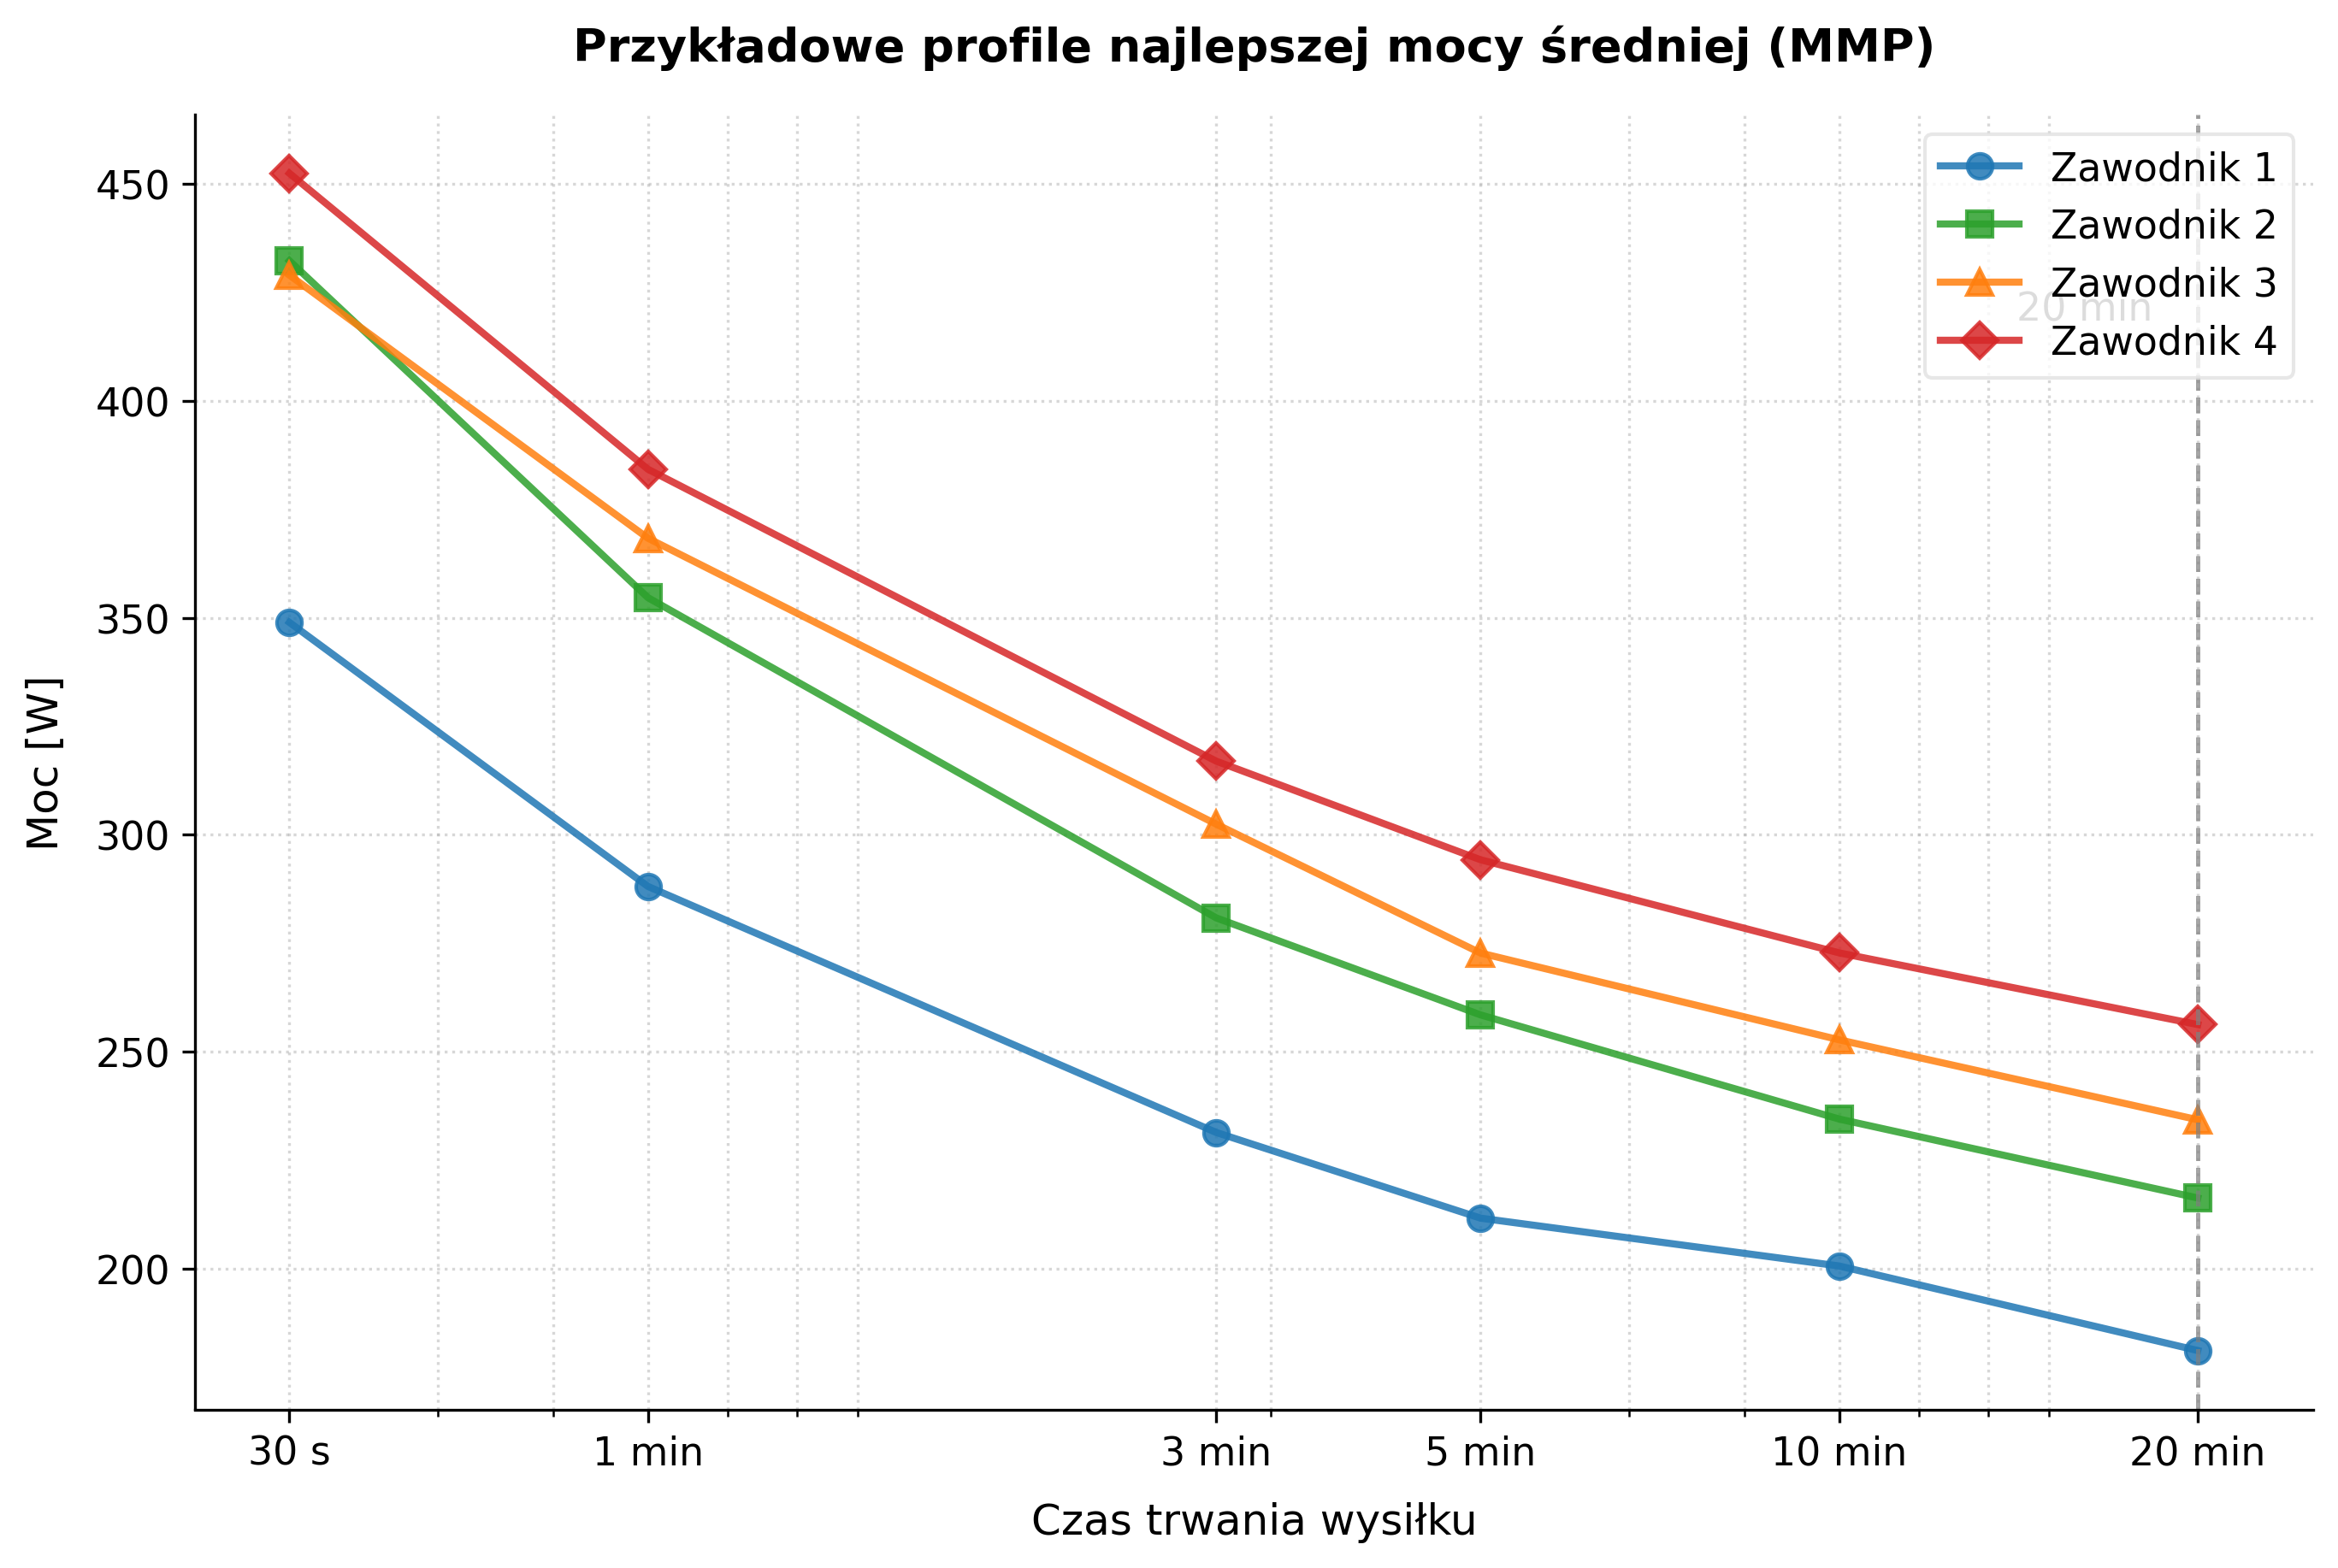
\includegraphics[width=0.85\textwidth]{figures/theory/power_duration_profiles_examples.png}
    \caption{Przykładowe profile mocy względem czasu trwania wysiłku}
    \label{fig:power_duration_profiles_examples}
    \figsource{Opracowanie własne na podstawie danych GoldenCheetah OpenData \parencite{osf_goldencheetah_opendata}.}
\end{figure}

Wykres ten pełni rolę empirycznego tła metodologicznego: pokazuje różnorodność i indywidualną charakterystykę profili wydolnościowych u różnych kolarzy. Ilustruje to potrzebę uwzględnienia różnic w profilach podczas trenowania modeli regresyjnych.

\section{Inżynieria cech}

Z szeregów czasowych wyznaczono zagregowane predyktory opisujące charakter sesji:
\begin{itemize}
    \item \textbf{Cechy czasu i objętości:} czas aktywności, czas jazdy bez przestojów, dystans i przewyższenie.
    \item \textbf{Cechy mocy:} średnia moc, percentyle rozkładu mocy, moc znormalizowana oraz histogramy intensywności.
    \item \textbf{Cechy tętna:} wartości średnie, maksymalne i miary zmienności.
    \item \textbf{Cechy kadencji:} statystyki rytmu pedałowania oraz udział fragmentów jazdy bez generowania mocy.
    \item \textbf{Cechy odsprzężenia tętna:} zmiany relacji pomiędzy mocą a tętnem w trakcie wysiłku.
    \item \textbf{Cechy Maximum Mean Power (MMP):} maksymalne średnie moce wyznaczane dla różnych długości okna czasowego, w tym \texttt{mmp\_20min}.
\end{itemize}

Histogramy intensywności i udziały czasu w zakresach mocy zachowują więcej informacji niż pojedyncza średnia. Dwie sesje o tej samej średniej mocy mogą mieć zupełnie inny przebieg: jedna może być równą jazdą wytrzymałościową, a druga zbiorem krótkich interwałów rozdzielonych odpoczynkiem. Podobnie kwantyle rozkładu pozwalają odróżnić poziom typowego obciążenia od wartości osiąganych jedynie okresowo.

Cechy odsprzężenia opisują zmianę relacji mocy do tętna w czasie. Jeżeli przy zbliżonym obciążeniu mechanicznym tętno stopniowo rośnie, może to wskazywać na dryf układu krążenia związany z czasem trwania wysiłku, temperaturą, odwodnieniem lub zmęczeniem. Wskaźniki te nie mają jednoznacznej interpretacji przyczynowej, lecz dostarczają modelowi informacji niedostępnej w samych statystykach mocy.

Cechy \texttt{mmp\_*} opisują maksymalną średnią moc utrzymywaną w oknach o różnych długościach. Są użyteczne, ponieważ przybliżają kształt krzywej mocy zawodnika, ale wymagają szczególnej ostrożności. \texttt{mmp\_20min} jest bezpośrednio używane podczas tworzenia etykiety i dlatego musi zostać usunięte z głównego wariantu badawczego. Pozostałe cechy MMP nie są identyczne z etykietą, lecz nadal pozostają blisko powiązane z profilem wydolności. Z tego powodu oceniono także wariant konserwatywny bez całej tej grupy.

\section{Warianty eksperymentalne}

W celu oceny wpływu cech MMP oraz identyfikacji ryzyka data leakage przygotowano trzy warianty:
\begin{enumerate}
    \item \textbf{Wariant A (kontrolny z ryzykiem data leakage):} zawiera cechę \texttt{mmp\_20min}, z której bezpośrednio obliczana jest etykieta FTP. Wariant służy wyłącznie diagnozie skutków wycieku informacji.
    \item \textbf{Wariant B (główny wariant badawczy):} zawiera 46 cech po usunięciu \texttt{mmp\_20min}. Jest podstawą oceny jakości modeli.
    \item \textbf{Wariant C (konserwatywny):} zawiera 41 cech po usunięciu wszystkich predyktorów z prefiksem \texttt{mmp\_}. Pozwala ocenić przydatność pozostałych informacji telemetrycznych.
\end{enumerate}

Wariant B usuwa bezpośredni składnik wzoru etykietującego, czyli \texttt{mmp\_20min}, lecz nie eliminuje całej informacji wynikającej z krzywej mocy zawodnika. Inne cechy MMP, na przykład \texttt{mmp\_10min} lub \texttt{mmp\_30min}, mogą nadal pełnić funkcję silnych pośrednich proxy etykiety FTP. Z tego powodu wariant C potraktowano jako bardziej konserwatywną ocenę zdolności predykcyjnej cech pośrednich, niewykorzystujących bezpośrednio rodziny cech MMP.

Porównanie wariantów nie służy wyborowi dowolnego zestawu dającego najniższy błąd. Każdy wariant odpowiada odrębnemu pytaniu metodologicznemu. Wariant A pokazuje, jak wygląda rezultat obciążony data leakage. Wariant B sprawdza, czy po usunięciu bezpośredniej składowej etykiety zachowana zostaje wysoka jakość predykcji. Wariant C ocenia, ile informacji pozostaje w telemetrii po bardziej rygorystycznym usunięciu predyktorów związanych z krzywą MMP. Dopiero wspólna interpretacja trzech konfiguracji pozwala ocenić źródła jakości modelu.

\section{Strategia podziału danych}

Losowy podział pojedynczych rekordów mógłby prowadzić do sytuacji, w której sesje tego samego zawodnika znalazłyby się jednocześnie w zbiorze treningowym i testowym, co grozi wystąpieniem data leakage, konfundowaniem tożsamości i fałszywie optymistyczną oceną jakości na etapie walidacji \parencite{kohavi1995cv,saeb2017useCase,chaibubNeto2019identity,tougui2021crossValidation,rosenblatt2024leakage,richter2021sportsMl}. Ograniczono to ryzyko przez zastosowanie mechanizmu \texttt{GroupShuffleSplit} \parencite{sklearn_groupkfold} z grupowaniem po identyfikatorze \texttt{athlete\_id}. Każdy zawodnik został przypisany wyłącznie do jednego podzbioru. Finalny eksperyment wykorzystywał pojedynczy podział treningowy i testowy z parametrami \texttt{test\_size=0.2} oraz \texttt{random\_state=42}.

Stabilność wyników dla różnych składów próby testowej mogłaby zostać w przyszłości oceniona przez powtarzany \texttt{GroupShuffleSplit} lub \texttt{GroupKFold}. Obecny pojedynczy podział nadal jest właściwszy niż losowe mieszanie sesji, ponieważ ogranicza wyciek informacji osobniczej.

Zwykły losowy split byłby błędny z punktu widzenia docelowego zastosowania. Sesje jednej osoby są ze sobą powiązane: mają podobny zakres mocy, charakterystyczną relację mocy do tętna, powtarzalne trasy i nawyki treningowe. Umieszczenie części aktywności tej samej osoby w treningu i teście umożliwiałoby modelowi korzystanie z tego profilu. Metryki opisywałyby wówczas przewidywanie kolejnej sesji zawodnika częściowo znanego algorytmowi, a nie generalizację na nową osobę.

Rysunek~\ref{fig:leakage_subject_split} syntetycznie pokazuje różnicę pomiędzy losowym podziałem sesji a podziałem osobniczym. Diagram nie dodaje nowego wariantu eksperymentu, lecz porządkuje przyjęte zabezpieczenie metodologiczne.

\begin{figure}[htbp]
\centering
\resizebox{\textwidth}{!}{%
\begin{tikzpicture}[
  node distance=0.42cm,
  box/.style={draw, rounded corners, align=center, minimum height=0.86cm, text width=5.9cm, fill=gray!8},
  warn/.style={draw, rounded corners, align=center, minimum height=0.86cm, text width=5.9cm, fill=red!8},
  ok/.style={draw, rounded corners, align=center, minimum height=0.86cm, text width=5.9cm, fill=green!8},
  arrow/.style={-{Stealth[length=2.4mm]}, thick}
]
\node[box] (sessions) {Wiele sesji tego samego zawodnika};

\node[warn, below left=0.8cm and 0.3cm of sessions] (randomsplit) {Losowy podział sesji};
\node[warn, below=of randomsplit] (sameathlete) {Ten sam \texttt{athlete\_id} może trafić do train i test};
\node[warn, below=of sameathlete] (optimistic) {Ryzyko leakage: model rozpoznaje profil znanego zawodnika};

\node[ok, below right=0.8cm and 0.3cm of sessions] (groupsplit) {Podział po zawodnikach};
\node[ok, below=of groupsplit] (separate) {Każdy \texttt{athlete\_id} występuje tylko w train albo tylko w test};
\node[ok, below=of separate] (generalization) {Ocena generalizacji na nieznanych zawodników};

\draw[arrow] (sessions) -- (randomsplit);
\draw[arrow] (randomsplit) -- (sameathlete);
\draw[arrow] (sameathlete) -- (optimistic);

\draw[arrow] (sessions) -- (groupsplit);
\draw[arrow] (groupsplit) -- (separate);
\draw[arrow] (separate) -- (generalization);
\end{tikzpicture}
%
}
\caption{Porównanie losowego podziału sesji i podziału osobniczego}
\label{fig:leakage_subject_split}
\figsource{Opracowanie własne.}
\end{figure}

Schemat ten graficznie porządkuje proces podziału danych, ułatwiając zrozumienie, dlaczego podział osobniczy chroni przed fałszywym zawyżeniem wyników walidacji.

Podział po \texttt{athlete\_id} stawia przed modelem trudniejsze i bardziej użyteczne zadanie. Każda predykcja testowa dotyczy sesji zawodnika, którego dane nie były wykorzystywane podczas uczenia. Nie eliminuje to wszystkich źródeł błędu ani nie zastępuje walidacji na zbiorze zewnętrznym, ale ogranicza jeden z najważniejszych rodzajów wycieku w danych wielosesyjnych.

\section{Modele i metryki oceny}

W eksperymencie porównano trzy modele regresyjne:
\begin{itemize}
    \item \textbf{Ridge Regression:} model liniowy z regularyzacją, pełniący funkcję punktu odniesienia \parencite{hoerl1970ridge}.
    \item \textbf{Random Forest:} model zespołowy oparty na uśrednianiu predykcji wielu drzew decyzyjnych \parencite{breiman2001random}.
    \item \textbf{XGBoost:} implementacja Gradient Boosting, w której kolejne drzewa korygują błędy wcześniejszych predykcji \parencite{chen2016xgboost}.
\end{itemize}

Jako miary jakości wykorzystano Mean Absolute Error (MAE), Root Mean Squared Error (RMSE), medianowy błąd bezwzględny (MedAE) oraz coefficient of determination ($R^2$). Metryki obliczano na zbiorze testowym złożonym z sesji zawodników nieobecnych w zbiorze treningowym \parencite{chai2014rmseMae}.

MAE jest podstawową miarą interpretowalną praktycznie, ponieważ opisuje przeciętną bezwzględną różnicę pomiędzy etykietą a predykcją w watach. RMSE również ma jednostkę watów, ale przez podnoszenie błędów do kwadratu silniej reaguje na większe pomyłki. Zestawienie obu miar pozwala zauważyć, czy poza typowymi błędami występują obserwacje wyraźnie trudniejsze dla modelu.

MedAE jest medianą bezwzględnych różnic i w mniejszym stopniu podlega wpływowi obserwacji odstających. Uzupełnia MAE, pokazując błąd typowy dla środkowej części rozkładu. Współczynnik $R^2$ informuje natomiast, jaka część zmienności etykiety jest odtwarzana przez predykcję względem prostego punktu odniesienia opartego na średniej. Nie należy interpretować go samodzielnie: wysoka wartość $R^2$ może współwystępować z data leakage, dlatego musi być analizowana łącznie z definicją cech, podziałem danych i błędem wyrażonym w watach.

\section{Wykorzystane technologie i narzędzia}

Implementację potoku przygotowano w języku Python. Do przetwarzania tabelarycznych danych sesji wykorzystano bibliotekę \texttt{pandas}, natomiast operacje numeryczne i obliczenia pomocnicze realizowano z użyciem biblioteki \texttt{NumPy}. Modele Ridge Regression i Random Forest, podział \texttt{GroupShuffleSplit}, imputację braków danych, standaryzację oraz obliczanie metryk regresyjnych zaimplementowano za pomocą biblioteki \texttt{scikit-learn} \parencite{pedregosa2011scikitLearn}. Model Gradient Boosting uruchamiano przy użyciu biblioteki \texttt{XGBoost}.

Wykresy wykorzystywane podczas analizy wyników generowano programowo z użyciem biblioteki \texttt{matplotlib}. Poszczególne etapy przygotowania danych i ewaluacji zostały rozdzielone pomiędzy skrypty potoku ETL. Taka organizacja pozwala powtarzać eksperymenty na tym samym zbiorze wejściowym, zachować jawne parametry podziału danych oraz odtworzyć kolejne etapy prowadzące od surowych archiwów do plików wynikowych.

\section{Podsumowanie}

Przyjęta metodologia umożliwia odtworzenie eksperymentu na podstawie przygotowanych skryptów i plików wynikowych. Kluczowe znaczenie mają dwa zabezpieczenia: osobniczy podział danych z wykorzystaniem \texttt{GroupShuffleSplit} oraz rozdzielenie wariantów A, B i C, które pozwala odróżnić wynik obciążony data leakage od głównego wyniku badawczego.

Należy podkreślić, że zmienna celu (\texttt{ftp\_label}) ma charakter operacyjny i heurystyczny. Została zdefiniowana jako $0{,}95$ maksymalnej średniej mocy 20-minutowej, a nie na podstawie kontrolowanego pomiaru laboratoryjnego. Model estymuje zatem przyjętą etykietę FTP, nie bezpośrednio mierzony próg fizjologiczny, taki jak moc krytyczna czy maksymalny stan równowagi mleczanowej. Interpretacja wyników musi uwzględniać to ograniczenie: wysoka jakość predykcji oznacza dobre przybliżenie heurystycznej wartości referencyjnej, a nie równoważność z diagnostyką laboratoryjną.
